\section{Approach}
\label{sec:approach}

In this section, we describe our model, which generates word vectors for cause and effect role simultaneously. 

\subsection{Causal Corpus Extraction}
\begin{table}[th]
	\centering
	\caption{Part of Causal cues. \textit{A} is a cause span, and \textit{B} is an effect span.}
	\label{tab:cue}
	\resizebox {0.5\textwidth}{!}{
		\begin{tabular}{|l l l|}
			\hline \multicolumn{3}{|c|}{intra-sentence}\\
			\hline \hline
			A lead to B & A give rise to B & A induce B\\
			A cause B & A bring on B & result from B  \\
			\multicolumn{3}{|c|}{......}\\
			\hline
			\multicolumn{3}{|c|}{inter-sentence}\\
			\hline \hline
			If A, then B & B because of A & A, thus B \\
			A, therefore B & In consequence of A, B & Due to B, A\\
			\multicolumn{3}{|c|}{......}\\
			\hline
	\end{tabular}}
\end{table}
At the beginning, we extract sentences containing causal knowledge using causal patterns by using the templates provided by Luo et al.~\cite{luo2016commonsense}. Several cues we used are shown in Table~\ref{tab:cue} One such sentence with $m+n+k$ words where $m$ is the length of cause span, $n$ is the length of effect span and $k$ is the length of causal cue, is denoted as $S = \langle w_1, ..., w_m, w_1, \dots, w_k, w_1, \dots, w_n\rangle$. Causal cue splits the sentence into cause and effect spans, which we name it one causal span pair.  
For sentences in Section 1, ``cause(d)'' is the causal cue which splits the sentence as follows:\\

\begin{enumerate}[(1)]
\item \underline{In 1998 the Pont du Gard was hit by major}  \underline{flooding which} [\emph{cause span}] \textbf{caused}  [\emph{pattern}] \underline{widespread damage in the area.} [\emph{effect span}]\\
\item \underline{Rainfall is occurring as heavy downpours that} [\emph{cause span}] {\bf cause} [\emph{pattern}] \underline{flooding.} [\emph{effect span}]
\end{enumerate}

We get two causal span pairs: (``In 1998 the Pont du Gard was hit by major flooding which'', ``widespread damage in the area.'') and (``Rainfall is occurring as heavy downpours that'', ``flooding.'').

We also consider the situation where only one word can not decribe a complete event, such as ``give up'' in sentence ``Don't \emph{give up} on love because of a bad exprience with a sleazy internet site.'' So we include the verbal phrases in our vocabulary. We use fuzzy match in the corpus so we can catch ``give up'' from ``give it up''.

\subsection{Vector Representation} 
\label{subsec:vec repre}

\begin{figure*}[!th]
	\centering
	%\epsfig{file=causalnet.eps, width=0.6\columnwidth}
	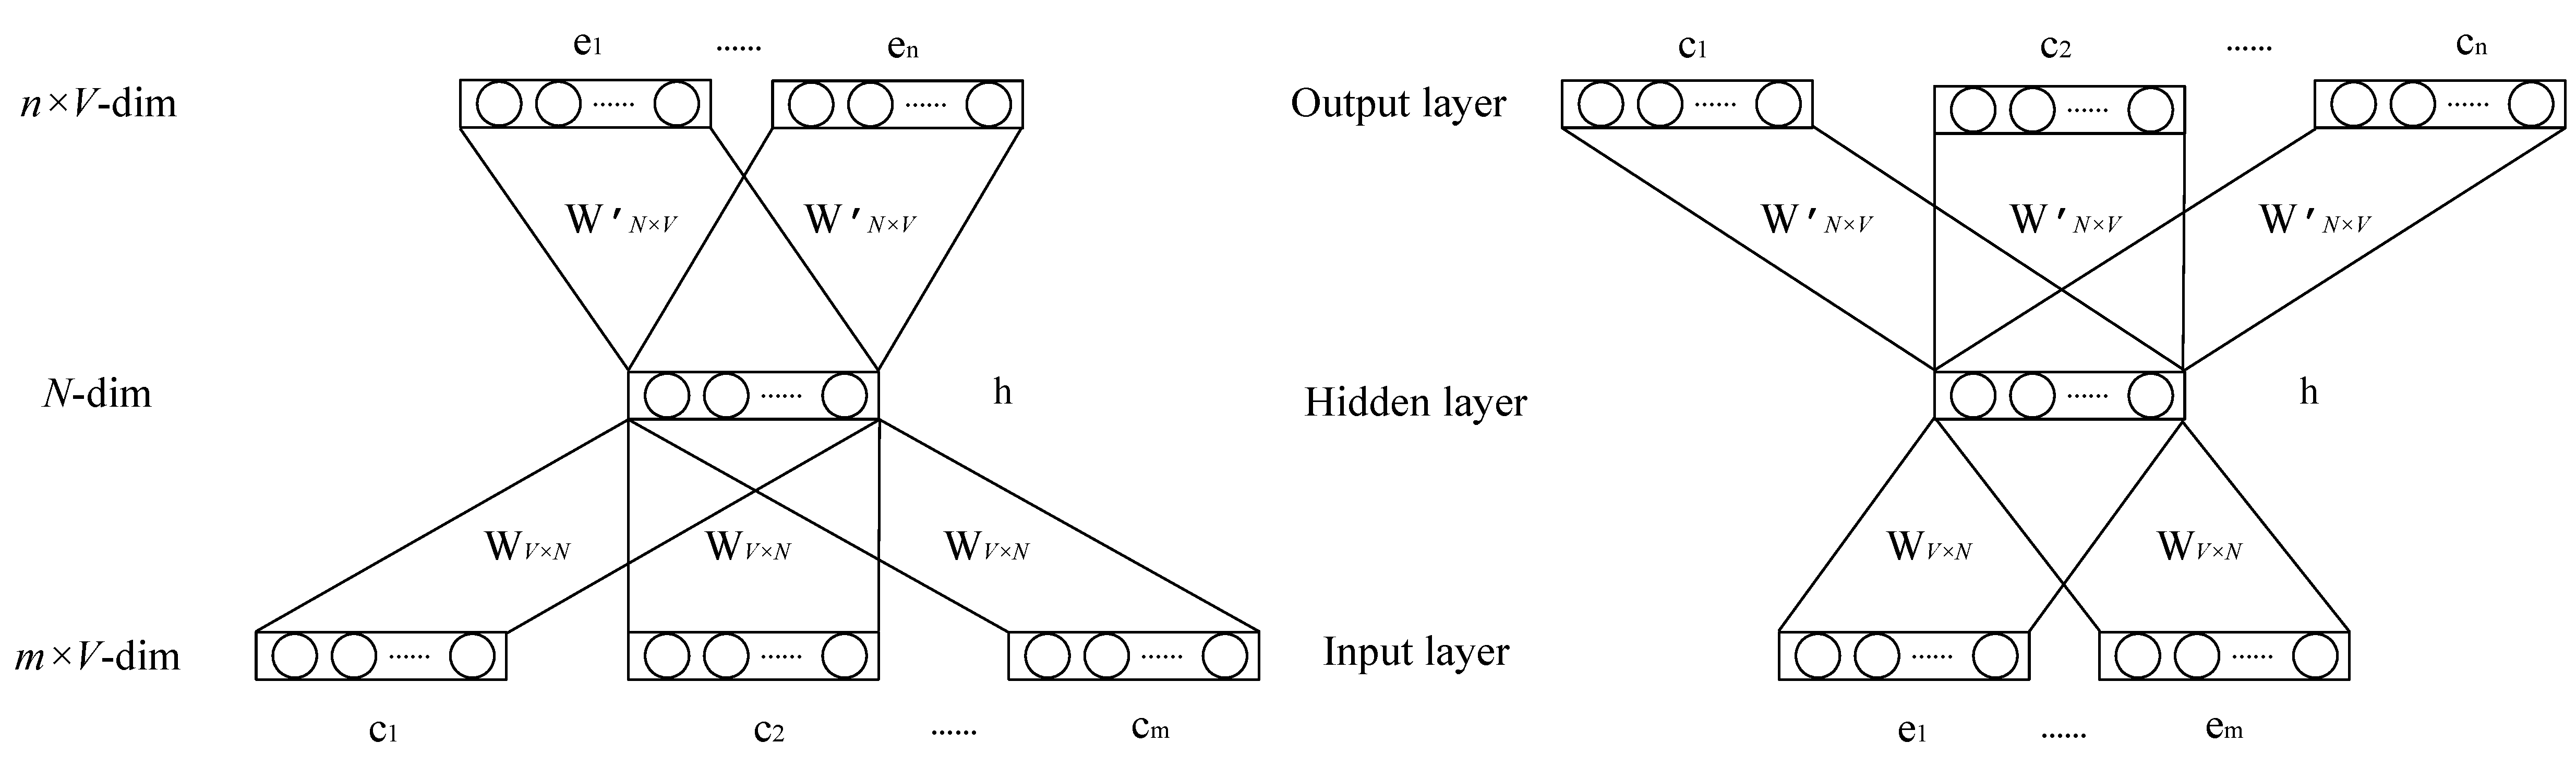
\includegraphics[width=2\columnwidth]{model}
	\caption{Model of Causal Embedding}
	\label{fig:model}
\end{figure*}

We modify the idea of word2vec \cite{mikolov2013distributed} by using cause span to predict the relative effect span and vice versa(\ref{fig:model}). Specifically, for word $w_i$, vector for cause role of this word is denoted as $\overrightarrow{c_i}$ and vector for effect role is denoted as $\overrightarrow{e_i}$. For any causal span pair, we use $C_{1 \sim m}$  and $E_{1 \sim n}$  to represent the context of cause and effect span. And the corresponding vector representations are $\overrightarrow{C_{1 \sim m}}$ and  $\overrightarrow{E_{1 \sim n}}$ where 

\begin{subequations}
	\label{eqs:contextRep}
	\begin{sequation}
	\overrightarrow{C_{1 \sim m}} = \frac{1}{m} \sum_{i=1}^m{\overrightarrow{c_i}}
	\end{sequation}
	\begin{sequation}
	\overrightarrow{E_{1 \sim n}} = \frac{1}{n} \sum_{i=1}^n{\overrightarrow{e_i}}
	\end{sequation}
\end{subequations}

We choose the straightforward way to represent span by averaging all word vectors in the span. It works both for the CBOW model of Word2vec and our work.
As introduced by Luo~\cite{luo2016commonsense}, causality between events appear in both sufficiency and necessity ways. In the example~\ref{eg:sen}, causal pair (\emph{flooding}, \emph{damage}) encodes more of sufficiency causality because the effect \emph{damage} can happen by not only making \emph{flooding} as its cause. Similarly, causal pair (\emph{rainfall}, \emph{flooding}) encodes more of necessity causality.
Consider the possibility of sentence $S$ being one that contains causality given causal or effect span, we estimate the probability from both necessity and sufficiency sides. 
To simplify the problem, we suppose that \emph{all words of the other span are generated conditionally independent}. Thus, we have:

\begin{subequations}
	\label{eqs:prob}
	\begin{sequation}
		\begin{aligned}
			P_{nec}(S) &= P(C_{1 \sim m}|E_{1 \sim n})\\
			&= P(c_1, c_2, ..., c_m|E_{1 \sim n}) = \prod_{i=1}^{m}{P(c_i|E_{1 \sim n})}  \\
		\end{aligned}
	\end{sequation}
	\begin{sequation}
		\begin{aligned}
			P_{suf}(S) &= P(E_{1 \sim n}|C_{1 \sim m})\\
			&= P(e_1, e_2, ..., e_n|C_{1 \sim m}) = \prod_{j=1}^{n}{P(e_j|C_{1 \sim m})} \\
		\end{aligned}
	\end{sequation}
\end{subequations}


Modify the idea of CBOW(Continuous Bag Of Words) in word2vec and the negative sampling algorithm, we then define the objective function as follows:

\begin{subequations}
	\label{eqs:loss}
	\begin{sequation}
	\label{eqs:loss_suf}
	\begin{aligned}
	l_{suf} &= -\log P_{suf}(S) = - \sum_{j=1}^{n}{\log P(e_j|C_{1 \sim m})} \\
	&= - \sum_{j=1}^{n}{\log \frac{exp(\overrightarrow{e_j} \cdot \overrightarrow{C_{1 \sim m}} )}{\sum_{w=1}^{W}{exp(\overrightarrow{e_w} \cdot \overrightarrow{C_{1 \sim m}})}}} \\
	&= -\sum_{j=1}^{n}{[\log\sigma(\overrightarrow{e_j} \cdot \overrightarrow{C_{1 \sim m}})} + \sum_{k=1}^{K}{\log(1 - \sigma(\overrightarrow{e_k} \cdot \overrightarrow{C_{1 \sim m}}))}]\\	
	\end{aligned}
	\end{sequation}
	\begin{sequation}
		\label{eqs:loss_nec}
		\begin{aligned}
		l_{nec} &= -\log P_{nec}(S) = -\sum_{i=1}^{m}{\log P(c_i|E_{1 \sim n})} \\
		&= - \sum_{i=1}^{m}{\log \frac{exp(\overrightarrow{c_i} \cdot \overrightarrow{E_{1 \sim n}} )}{\sum_{w=1}^{W}{exp(\overrightarrow{c_w} \cdot \overrightarrow{E{1 \sim n}})}}} \\
		&= -\sum_{i=1}^{m}{[\log\sigma(\overrightarrow{c_i} \cdot \overrightarrow{E_{1 \sim n}})} + \sum_{k=1}^{K}{\log(1- \sigma(\overrightarrow{c_k} \cdot \overrightarrow{E_{1 \sim n}}))}] \\
		\end{aligned}
	\end{sequation}
	
\end{subequations}

We use softmax to formulate the probability given one span predicting the word of the other span(line 1-2 of the equation~\ref{eqs:loss}). $W$ is the size the whole vocabulary. It is very time-consuming to directly calculate the probability so we use negative sampling(line 2-3 of the equation~\ref{eqs:loss}) to model the log probability. $K$ is the number of negative samples. On one side, we hope the dot product of the correct word and span is as large as possible. On the other side, we hope the sampled wrong words are as far as possible away from the span. We choose the noise distribution used by Mikolov et al. \cite{mikolov2013distributed} in the sampling which is unigram distribution raised to $3/4$rd power. 

We have two loss functions towarding cause or effect span as premise, so we get two sets of word matrixes finally: one of which pays more attention to the cause role while the other concentrates on the effect role. We define them as sufficiency set $(W_c, W_{eneg})$ and necessity set $(W_{cneg}, W_e)$ where each of them models the sufficiency and necessity of causality respectively. 
More specificlly, in sufficiency part(equation~(\ref{eqs:loss_suf})), vectors representing cause span($\overrightarrow{C_{1\sim m}}$) are from the matrix $W_c$ while vectors($\overrightarrow{e_k}$) representing the effect words are sampled from $W_{eneg}$. Similarly, in neccessity part(equation~(\ref{eqs:loss_nec})), vectors used for calculating $\overrightarrow{E_{1\sim n}}$ are from matrix $W_e$ and vectors representing possible cause($\overrightarrow{c_k}$) are sampled from $W_{cneg}$. We use \emph{neg} here because those word embeddings are used as negative samples in the equations.
%Besides, we define the causal strength as the cosine similarity between word vectors of two roles.


\subsection{Causal Strength}
We can now calculate the causal strength between two words by using these vectors.
Similar to word2vec, we use the dot product of two vectors(Equation~\ref{eq:cs}). 
We have two sets of embedding corresponding to different causal spaces. We can then combine them together like Eqaution~\ref{eq:cs3}.

\begin{subequations}
	\centering
	\label{eq:cs}
	\begin{equation}
	\begin{aligned}
	CS_{suf} &= \overrightarrow{c_i} \cdot \overrightarrow{e_j},\\
	& where\,\, \overrightarrow{c_i} \in W_c \,\, and \,\, \overrightarrow{e_j} \in W_{eneg} \\
	\end{aligned}
	\end{equation}
	\begin{equation}
	\begin{aligned}
	CS_{nec} &= \overrightarrow{c_i} \cdot \overrightarrow{e_j},\\
	& where\,\, \overrightarrow{c_i} \in W_{cneg} \,\, and \,\, \overrightarrow{e_j} \in W_{e} \\
	\end{aligned}
	\end{equation}
	\begin{equation}
	\label{eq:cs3}
	CS = \lambda CS_{suf} + (1-\lambda) CS_{nec}
	\end{equation}
\end{subequations}

The trick is that we can either normalize the vectors or not. As Schakel\cite{schakel2015measuring} discuessed in his paper, both the length and the direction of vectors in word2vec are meaningful. \emph{Context word}s which hold real meaning of the sentence, usually appear in limited contexts. And with the growth of frequency, the norm of vectors grows as well because they are updated to the only several directions. On the other hand, \emph{function word}s which are words used for organizing a sentence, appear evenly distributed across a corpus. They usually have high frequency but cooccur with many different words so they are updated to all the directions and the norm is not very large. 
In Word2Vec, we use the normalized vectors when calculating the similarity while the unnormalized one shows the ablity to linearize analogies. In our task, causal strength are calculated by both of the two ways.
Experiments show that they perform well in different situation.

\subsection{Discussion}
%the advatage of our method vs statistical method
Though we have good human-designed templates(Table~\ref{tab:cue}) for extracting causal span pairs, there is stilll possible that we get sentences without causal knowledge. For example: 
\begin{example}
	\noindent
	\begin{itemize}
		\item[(1)] \textbf{If} possible\textbf{,} restrict use to a low flash frequency.
		\item[(2)] Jack reached the door \textbf{leading to} one hall.
	\end{itemize}
\end{example}
As the example shows, templates can not always catch causal knowledge because some of them may have other meanings rather than indicate the causality. It is also hard to eliminate such noises unless using more complex semantic or syntactic methods which are time-consuming and not 100\% correct either.
The good news is that the noises have low frequency and with the increasing amount of text corpus, even very naive statistical method can somewhat reduce the influence of the noise as Luo~\cite{luo2016commonsense} does in his paper.
Our embedding meghod is even better, since using negative sampling, we not only drag correct pair closer but also push the wrong pairs away. Every time we update the vectors, it influences a subspace of the causal space.